\documentclass[twoside]{book}

% Packages required by doxygen
\usepackage{calc}
\usepackage{doxygen}
\usepackage{graphicx}
\usepackage[utf8]{inputenc}
\usepackage{makeidx}
\usepackage{multicol}
\usepackage{multirow}
\PassOptionsToPackage{warn}{textcomp}
\usepackage{textcomp}
\usepackage[nointegrals]{wasysym}
\usepackage[table]{xcolor}

% Font selection
\usepackage[T1]{fontenc}
\usepackage{mathptmx}
\usepackage[scaled=.90]{helvet}
\usepackage{courier}
\usepackage{amssymb}
\usepackage{sectsty}
\renewcommand{\familydefault}{\sfdefault}
\allsectionsfont{%
  \fontseries{bc}\selectfont%
  \color{darkgray}%
}
\renewcommand{\DoxyLabelFont}{%
  \fontseries{bc}\selectfont%
  \color{darkgray}%
}
\newcommand{\+}{\discretionary{\mbox{\scriptsize$\hookleftarrow$}}{}{}}

% Page & text layout
\usepackage{geometry}
\geometry{%
  a4paper,%
  top=2.5cm,%
  bottom=2.5cm,%
  left=2.5cm,%
  right=2.5cm%
}
\tolerance=750
\hfuzz=15pt
\hbadness=750
\setlength{\emergencystretch}{15pt}
\setlength{\parindent}{0cm}
\setlength{\parskip}{0.2cm}
\makeatletter
\renewcommand{\paragraph}{%
  \@startsection{paragraph}{4}{0ex}{-1.0ex}{1.0ex}{%
    \normalfont\normalsize\bfseries\SS@parafont%
  }%
}
\renewcommand{\subparagraph}{%
  \@startsection{subparagraph}{5}{0ex}{-1.0ex}{1.0ex}{%
    \normalfont\normalsize\bfseries\SS@subparafont%
  }%
}
\makeatother

% Headers & footers
\usepackage{fancyhdr}
\pagestyle{fancyplain}
\fancyhead[LE]{\fancyplain{}{\bfseries\thepage}}
\fancyhead[CE]{\fancyplain{}{}}
\fancyhead[RE]{\fancyplain{}{\bfseries\leftmark}}
\fancyhead[LO]{\fancyplain{}{\bfseries\rightmark}}
\fancyhead[CO]{\fancyplain{}{}}
\fancyhead[RO]{\fancyplain{}{\bfseries\thepage}}
\fancyfoot[LE]{\fancyplain{}{}}
\fancyfoot[CE]{\fancyplain{}{}}
\fancyfoot[RE]{\fancyplain{}{\bfseries\scriptsize Generated on Thu Apr 23 2015 14\+:25\+:32 for Easel by Doxygen }}
\fancyfoot[LO]{\fancyplain{}{\bfseries\scriptsize Generated on Thu Apr 23 2015 14\+:25\+:32 for Easel by Doxygen }}
\fancyfoot[CO]{\fancyplain{}{}}
\fancyfoot[RO]{\fancyplain{}{}}
\renewcommand{\footrulewidth}{0.4pt}
\renewcommand{\chaptermark}[1]{%
  \markboth{#1}{}%
}
\renewcommand{\sectionmark}[1]{%
  \markright{\thesection\ #1}%
}

% Indices & bibliography
\usepackage{natbib}
\usepackage[titles]{tocloft}
\setcounter{tocdepth}{3}
\setcounter{secnumdepth}{5}
\makeindex

% Packages requested by user
\usepackage{float}

% Hyperlinks (required, but should be loaded last)
\usepackage{ifpdf}
\ifpdf
  \usepackage[pdftex,pagebackref=true]{hyperref}
\else
  \usepackage[ps2pdf,pagebackref=true]{hyperref}
\fi
\hypersetup{%
  colorlinks=true,%
  linkcolor=blue,%
  citecolor=blue,%
  unicode%
}

% Custom commands
\newcommand{\clearemptydoublepage}{%
  \newpage{\pagestyle{empty}\cleardoublepage}%
}


%===== C O N T E N T S =====

\begin{document}

% Titlepage & ToC
\hypersetup{pageanchor=false,
             bookmarks=true,
             bookmarksnumbered=true,
             pdfencoding=unicode
            }
\pagenumbering{roman}
\begin{titlepage}
\vspace*{7cm}
\begin{center}%
{\Large Easel }\\
\vspace*{1cm}
{\large Generated by Doxygen 1.8.7}\\
\vspace*{0.5cm}
{\small Thu Apr 23 2015 14:25:32}\\
\end{center}
\end{titlepage}
\clearemptydoublepage
\tableofcontents
\clearemptydoublepage
\pagenumbering{arabic}
\hypersetup{pageanchor=true}

%--- Begin generated contents ---
\chapter{Hierarchical Index}
\section{Class Hierarchy}
This inheritance list is sorted roughly, but not completely, alphabetically\+:\begin{DoxyCompactList}
\item \contentsline{section}{cs.\+easel.\+Draw\+Path}{\pageref{classcs_1_1easel_1_1_draw_path}}{}
\item Activity\begin{DoxyCompactList}
\item \contentsline{section}{cs.\+easel.\+Draw\+Test}{\pageref{classcs_1_1easel_1_1_draw_test}}{}
\item \contentsline{section}{cs.\+easel.\+Launcher}{\pageref{classcs_1_1easel_1_1_launcher}}{}
\end{DoxyCompactList}
\item Surface\+View\begin{DoxyCompactList}
\item \contentsline{section}{cs.\+easel.\+Draw\+Panel}{\pageref{classcs_1_1easel_1_1_draw_panel}}{}
\end{DoxyCompactList}
\end{DoxyCompactList}

\chapter{Class Index}
\section{Class List}
Here are the classes, structs, unions and interfaces with brief descriptions\+:\begin{DoxyCompactList}
\item\contentsline{section}{\hyperlink{classcs_1_1easel_1_1_draw_panel}{cs.\+easel.\+Draw\+Panel} }{\pageref{classcs_1_1easel_1_1_draw_panel}}{}
\item\contentsline{section}{\hyperlink{classcs_1_1easel_1_1_draw_path}{cs.\+easel.\+Draw\+Path} }{\pageref{classcs_1_1easel_1_1_draw_path}}{}
\item\contentsline{section}{\hyperlink{classcs_1_1easel_1_1_draw_test}{cs.\+easel.\+Draw\+Test} }{\pageref{classcs_1_1easel_1_1_draw_test}}{}
\item\contentsline{section}{\hyperlink{classcs_1_1easel_1_1_launcher}{cs.\+easel.\+Launcher} }{\pageref{classcs_1_1easel_1_1_launcher}}{}
\end{DoxyCompactList}

\chapter{Class Documentation}
\hypertarget{classcs_1_1easel_1_1_draw_panel}{\section{cs.\+easel.\+Draw\+Panel Class Reference}
\label{classcs_1_1easel_1_1_draw_panel}\index{cs.\+easel.\+Draw\+Panel@{cs.\+easel.\+Draw\+Panel}}
}
Inheritance diagram for cs.\+easel.\+Draw\+Panel\+:\begin{figure}[H]
\begin{center}
\leavevmode
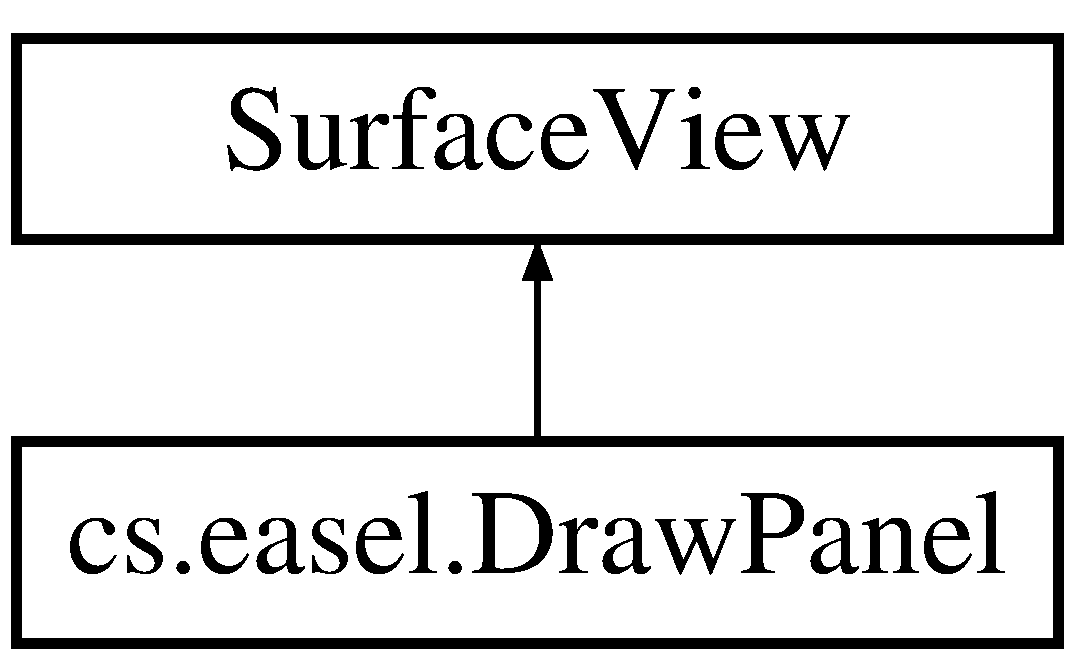
\includegraphics[height=2.000000cm]{classcs_1_1easel_1_1_draw_panel}
\end{center}
\end{figure}
\subsection*{Public Member Functions}
\begin{DoxyCompactItemize}
\item 
\hypertarget{classcs_1_1easel_1_1_draw_panel_aa363ca7d93536d3ad544f36668a8a4be}{double {\bfseries cosine\+Interpolation} (double x1, double x2, double normal)}\label{classcs_1_1easel_1_1_draw_panel_aa363ca7d93536d3ad544f36668a8a4be}

\item 
\hypertarget{classcs_1_1easel_1_1_draw_panel_ace5a2cc679d374f3142c833b3cb69f44}{{\bfseries Draw\+Panel} (Context context)}\label{classcs_1_1easel_1_1_draw_panel_ace5a2cc679d374f3142c833b3cb69f44}

\item 
\hypertarget{classcs_1_1easel_1_1_draw_panel_ad8a01a1b1abcc70e9e9e6cfea620f5c5}{{\bfseries Draw\+Panel} (Context context, Attribute\+Set attrs, int def\+Style)}\label{classcs_1_1easel_1_1_draw_panel_ad8a01a1b1abcc70e9e9e6cfea620f5c5}

\item 
\hypertarget{classcs_1_1easel_1_1_draw_panel_ae087cc858798731f1c746a45b15e6a4a}{{\bfseries Draw\+Panel} (Context context, Attribute\+Set attrs)}\label{classcs_1_1easel_1_1_draw_panel_ae087cc858798731f1c746a45b15e6a4a}

\item 
\hypertarget{classcs_1_1easel_1_1_draw_panel_a09054d42f615ea2169a74e86ca65e605}{void {\bfseries on\+Draw} (Canvas canvas)}\label{classcs_1_1easel_1_1_draw_panel_a09054d42f615ea2169a74e86ca65e605}

\item 
\hypertarget{classcs_1_1easel_1_1_draw_panel_a27d4dc58056d2608e58308be498797ed}{boolean {\bfseries on\+Touch\+Event} (Motion\+Event event)}\label{classcs_1_1easel_1_1_draw_panel_a27d4dc58056d2608e58308be498797ed}

\end{DoxyCompactItemize}
\subsection*{Static Public Member Functions}
\begin{DoxyCompactItemize}
\item 
\hypertarget{classcs_1_1easel_1_1_draw_panel_a31a81adc2fb73955a02cd0ef493c3047}{static void {\bfseries change\+Black} ()}\label{classcs_1_1easel_1_1_draw_panel_a31a81adc2fb73955a02cd0ef493c3047}

\item 
\hypertarget{classcs_1_1easel_1_1_draw_panel_a69e5b44fba43cb141a9c15caf157b0ec}{static void {\bfseries change\+Red} ()}\label{classcs_1_1easel_1_1_draw_panel_a69e5b44fba43cb141a9c15caf157b0ec}

\item 
\hypertarget{classcs_1_1easel_1_1_draw_panel_a6a186bdaddc7b3a01ee299d8f54ef04a}{static void {\bfseries change\+Green} ()}\label{classcs_1_1easel_1_1_draw_panel_a6a186bdaddc7b3a01ee299d8f54ef04a}

\item 
\hypertarget{classcs_1_1easel_1_1_draw_panel_ae03cd407d8c5c15d851277f66387e5b3}{static void {\bfseries change\+Blue} ()}\label{classcs_1_1easel_1_1_draw_panel_ae03cd407d8c5c15d851277f66387e5b3}

\item 
\hypertarget{classcs_1_1easel_1_1_draw_panel_a989814529888ecb48bcd16e8110ed72e}{static void {\bfseries erase} ()}\label{classcs_1_1easel_1_1_draw_panel_a989814529888ecb48bcd16e8110ed72e}

\end{DoxyCompactItemize}
\subsection*{Public Attributes}
\begin{DoxyCompactItemize}
\item 
\hypertarget{classcs_1_1easel_1_1_draw_panel_aeb6242ff8bdae21e8ea2d0cc8ec39f74}{Path {\bfseries path} = new Path()}\label{classcs_1_1easel_1_1_draw_panel_aeb6242ff8bdae21e8ea2d0cc8ec39f74}

\end{DoxyCompactItemize}
\subsection*{Static Public Attributes}
\begin{DoxyCompactItemize}
\item 
\hypertarget{classcs_1_1easel_1_1_draw_panel_abf7cab6befdb118811b734d480d2f0e0}{static int {\bfseries current\+Color} = Color.\+B\+L\+A\+C\+K}\label{classcs_1_1easel_1_1_draw_panel_abf7cab6befdb118811b734d480d2f0e0}

\end{DoxyCompactItemize}


The documentation for this class was generated from the following file\+:\begin{DoxyCompactItemize}
\item 
app/src/main/java/cs/easel/Draw\+Panel.\+java\end{DoxyCompactItemize}

\hypertarget{classcs_1_1easel_1_1_draw_path}{\section{cs.\+easel.\+Draw\+Path Class Reference}
\label{classcs_1_1easel_1_1_draw_path}\index{cs.\+easel.\+Draw\+Path@{cs.\+easel.\+Draw\+Path}}
}
\subsection*{Public Member Functions}
\begin{DoxyCompactItemize}
\item 
\hypertarget{classcs_1_1easel_1_1_draw_path_ac815ec0578e48bd32d26764635b00ab2}{{\bfseries Draw\+Path} (int start\+Width)}\label{classcs_1_1easel_1_1_draw_path_ac815ec0578e48bd32d26764635b00ab2}

\item 
\hypertarget{classcs_1_1easel_1_1_draw_path_a21ae81f4c01afc4336d83545364c5d32}{void {\bfseries set\+Width} (int new\+Width)}\label{classcs_1_1easel_1_1_draw_path_a21ae81f4c01afc4336d83545364c5d32}

\end{DoxyCompactItemize}
\subsection*{Public Attributes}
\begin{DoxyCompactItemize}
\item 
\hypertarget{classcs_1_1easel_1_1_draw_path_a01746d060493378ca7ec29c89bb9875d}{int {\bfseries width}}\label{classcs_1_1easel_1_1_draw_path_a01746d060493378ca7ec29c89bb9875d}

\end{DoxyCompactItemize}


\subsection{Detailed Description}
Created by Eric on 4/1/15. 

The documentation for this class was generated from the following file\+:\begin{DoxyCompactItemize}
\item 
app/src/main/java/cs/easel/Draw\+Path.\+java\end{DoxyCompactItemize}

\hypertarget{classcs_1_1easel_1_1_draw_test}{\section{cs.\+easel.\+Draw\+Test Class Reference}
\label{classcs_1_1easel_1_1_draw_test}\index{cs.\+easel.\+Draw\+Test@{cs.\+easel.\+Draw\+Test}}
}
Inheritance diagram for cs.\+easel.\+Draw\+Test\+:\begin{figure}[H]
\begin{center}
\leavevmode
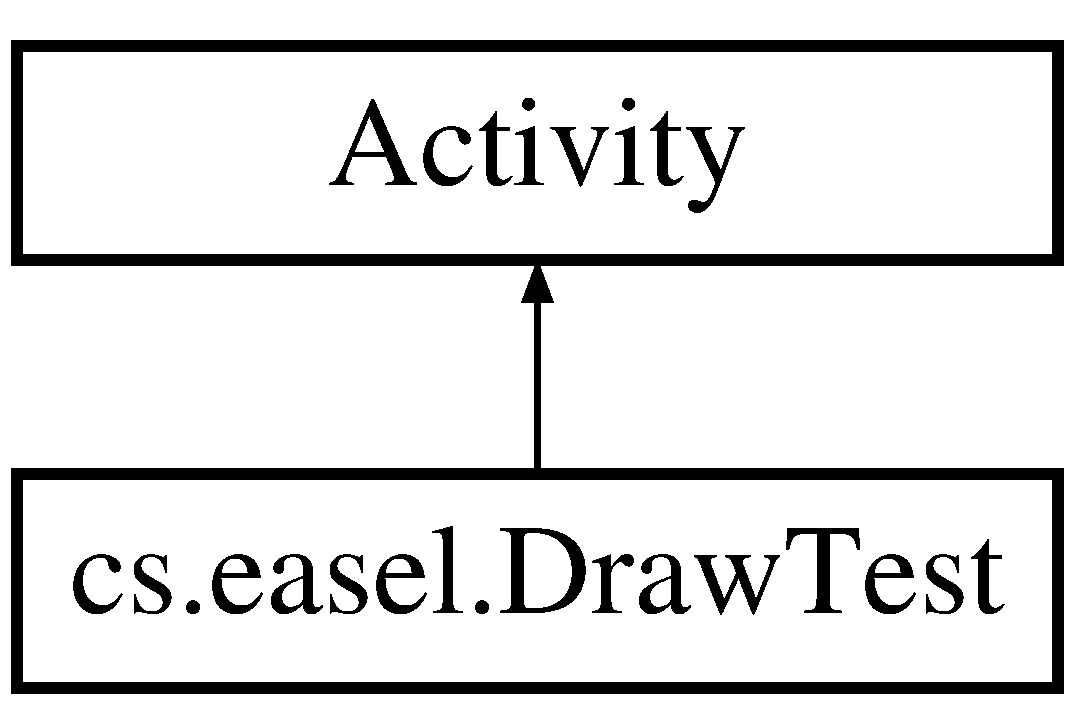
\includegraphics[height=2.000000cm]{classcs_1_1easel_1_1_draw_test}
\end{center}
\end{figure}
\subsection*{Public Member Functions}
\begin{DoxyCompactItemize}
\item 
\hypertarget{classcs_1_1easel_1_1_draw_test_a039580e2b2bd6628e4645c09f7691061}{boolean {\bfseries on\+Create\+Options\+Menu} (Menu menu)}\label{classcs_1_1easel_1_1_draw_test_a039580e2b2bd6628e4645c09f7691061}

\item 
\hypertarget{classcs_1_1easel_1_1_draw_test_a14ca9caff67166d1218da1f2eadeb06e}{boolean {\bfseries on\+Options\+Item\+Selected} (Menu\+Item item)}\label{classcs_1_1easel_1_1_draw_test_a14ca9caff67166d1218da1f2eadeb06e}

\item 
\hypertarget{classcs_1_1easel_1_1_draw_test_aa4451d77bc71016c1ee7780ac6430f13}{void {\bfseries red\+Button\+On\+Click} (View view)}\label{classcs_1_1easel_1_1_draw_test_aa4451d77bc71016c1ee7780ac6430f13}

\item 
\hypertarget{classcs_1_1easel_1_1_draw_test_a0bb178c4c7a4150ff1da220bc08d02ed}{void {\bfseries green\+Button\+On\+Click} (View view)}\label{classcs_1_1easel_1_1_draw_test_a0bb178c4c7a4150ff1da220bc08d02ed}

\item 
\hypertarget{classcs_1_1easel_1_1_draw_test_a22c03a4d88104dce37783b63fa7db681}{void {\bfseries blue\+Button\+On\+Click} (View view)}\label{classcs_1_1easel_1_1_draw_test_a22c03a4d88104dce37783b63fa7db681}

\item 
\hypertarget{classcs_1_1easel_1_1_draw_test_aba55091ae758713bbefd5ae7071e0021}{void {\bfseries black\+Button\+On\+Click} (View view)}\label{classcs_1_1easel_1_1_draw_test_aba55091ae758713bbefd5ae7071e0021}

\item 
\hypertarget{classcs_1_1easel_1_1_draw_test_a341a6c3968c3da92a5320df2874bbd3b}{void {\bfseries erase\+Button\+On\+Click} (View view)}\label{classcs_1_1easel_1_1_draw_test_a341a6c3968c3da92a5320df2874bbd3b}

\end{DoxyCompactItemize}
\subsection*{Protected Member Functions}
\begin{DoxyCompactItemize}
\item 
\hypertarget{classcs_1_1easel_1_1_draw_test_ad76a0e6568b82a0070545436c022bb49}{void {\bfseries on\+Create} (Bundle saved\+Instance\+State)}\label{classcs_1_1easel_1_1_draw_test_ad76a0e6568b82a0070545436c022bb49}

\end{DoxyCompactItemize}


The documentation for this class was generated from the following file\+:\begin{DoxyCompactItemize}
\item 
app/src/main/java/cs/easel/Draw\+Test.\+java\end{DoxyCompactItemize}

\hypertarget{classcs_1_1easel_1_1_launcher}{\section{cs.\+easel.\+Launcher Class Reference}
\label{classcs_1_1easel_1_1_launcher}\index{cs.\+easel.\+Launcher@{cs.\+easel.\+Launcher}}
}
Inheritance diagram for cs.\+easel.\+Launcher\+:\begin{figure}[H]
\begin{center}
\leavevmode
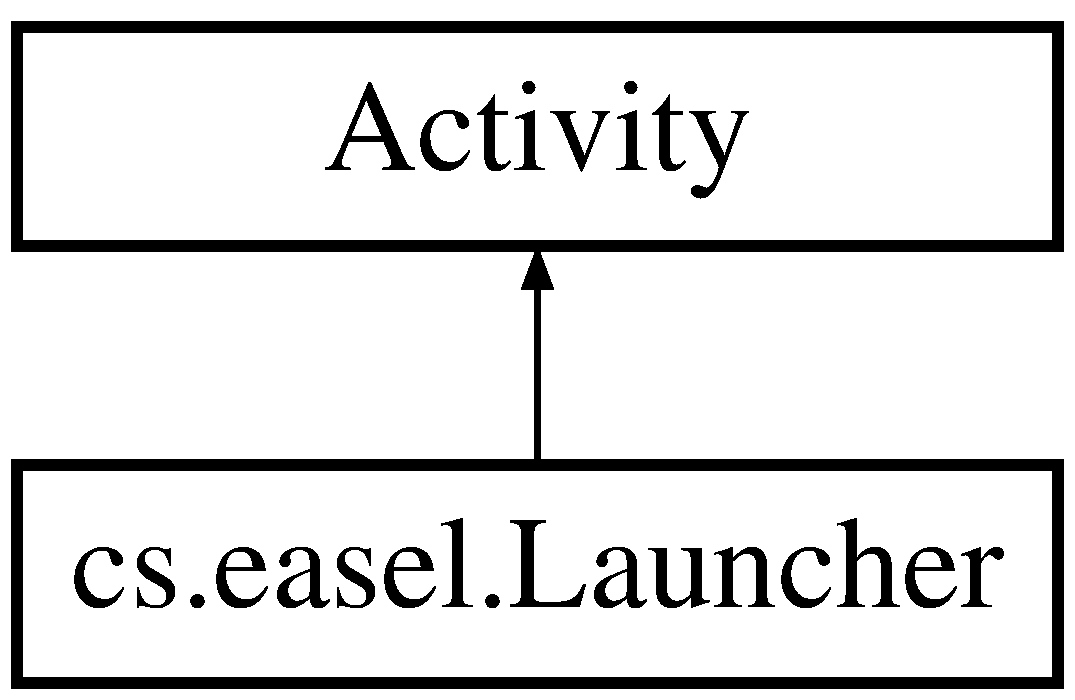
\includegraphics[height=2.000000cm]{classcs_1_1easel_1_1_launcher}
\end{center}
\end{figure}
\subsection*{Public Member Functions}
\begin{DoxyCompactItemize}
\item 
\hypertarget{classcs_1_1easel_1_1_launcher_a3a0753021e3d1510c4ebb6bb941b073c}{void {\bfseries button\+On\+Click} (View v)}\label{classcs_1_1easel_1_1_launcher_a3a0753021e3d1510c4ebb6bb941b073c}

\item 
\hypertarget{classcs_1_1easel_1_1_launcher_a60a9b20070e2aa8057de03ca8483efd0}{void {\bfseries button2\+On\+Click} (View v)}\label{classcs_1_1easel_1_1_launcher_a60a9b20070e2aa8057de03ca8483efd0}

\item 
\hypertarget{classcs_1_1easel_1_1_launcher_abad04c8d6b8aa20e931abbefe4031a09}{boolean {\bfseries on\+Create\+Options\+Menu} (Menu menu)}\label{classcs_1_1easel_1_1_launcher_abad04c8d6b8aa20e931abbefe4031a09}

\item 
\hypertarget{classcs_1_1easel_1_1_launcher_a236c7804113abde51fcef61cec2e82e7}{boolean {\bfseries on\+Options\+Item\+Selected} (Menu\+Item item)}\label{classcs_1_1easel_1_1_launcher_a236c7804113abde51fcef61cec2e82e7}

\end{DoxyCompactItemize}
\subsection*{Static Public Attributes}
\begin{DoxyCompactItemize}
\item 
\hypertarget{classcs_1_1easel_1_1_launcher_aa6e4b63807c96d9635e5677ed4c026d5}{static final String {\bfseries E\+X\+T\+R\+A\+\_\+\+M\+E\+S\+S\+A\+G\+E} = \char`\"{}com.\+mycompany.\+myfirstapp.\+M\+E\+S\+S\+A\+G\+E\char`\"{}}\label{classcs_1_1easel_1_1_launcher_aa6e4b63807c96d9635e5677ed4c026d5}

\end{DoxyCompactItemize}
\subsection*{Protected Member Functions}
\begin{DoxyCompactItemize}
\item 
\hypertarget{classcs_1_1easel_1_1_launcher_a2f03cb72c4c991de9d8530f4c359f625}{void {\bfseries on\+Create} (Bundle saved\+Instance\+State)}\label{classcs_1_1easel_1_1_launcher_a2f03cb72c4c991de9d8530f4c359f625}

\end{DoxyCompactItemize}


The documentation for this class was generated from the following file\+:\begin{DoxyCompactItemize}
\item 
app/src/main/java/cs/easel/Launcher.\+java\end{DoxyCompactItemize}

%--- End generated contents ---

% Index
\newpage
\phantomsection
\addcontentsline{toc}{chapter}{Index}
\printindex

\end{document}
